% Author: LeyuDame
% Date: 2024-04-20
% Github: https://github.com/LeyuDame/BNUslides
% Overleaf: 

% !TeX program = xelatex*2
\documentclass{bnuslides}
\begin{document}
\frame[plain]{\titlepage}
\frame[plain]{\frametitle{目录}\tableofcontents}

\section{模板介绍}
\subsection{制作愿景}
\begin{frame}{制作愿景}
	\begin{enumerate}
		\item 看起来专业一些: 主要适合理工科尤其数学的pre(例如毕业答辩),比如选用了清晰明了的信息栏与侧栏目录以及好看的数学字体
		\item 用起来简单一些:编译方式为\texttt{xelatex*2}, 不需要的功能一个没有,甚至省去了\texttt{bib}引用,可按需自行添加其他功能
		\item 师大蓝纯正一些:后面有讲
	\end{enumerate}
\end{frame}

\subsection{主要特色}
\begin{frame}{主要特色}
	\begin{enumerate}
		\item 纯粹的师大蓝:两种颜色分别取自官网和校徽,再设置不同透明度进行组合
		\item 极致的矢量图:可以直接使用Tikz作图,包括封面校徽logo
		\item 数学字体选用了Fourier
		\item 与图书馆官方毕业论文模板语法一致,制作答辩slides可以实现无缝迁移,例如$\symbf{r},\uppi,\dif x$
		\item 采用了16:9的显示比例而非传统的4:3,更适用于电脑和投影仪上展示,并加入了侧栏目录设计
		\item 用\texttt{.cls}文件单独控制格式,实现内容与格式完全分离
	\end{enumerate}
\end{frame}

\section{功能演示}
\subsection{列表}
\begin{frame}{分栏与编号}
	\begin{multicols}{2}
		有编号列表
		\begin{enumerate}
			\item  $\alpha$
			\item  $\beta$
			\item $\gamma$
		\end{enumerate}

		无编号列表
		\begin{itemize}
			\item   \texttt{\textbackslash alpha}
			\item  \texttt{\textbackslash beta}
			\item             \texttt{\textbackslash gamma}
		\end{itemize}
	\end{multicols}
\end{frame}

\subsection{插图}
\begin{frame}{Tikz插图}
	可以通过Tikz进行绘图, 例如
	\begin{figure}[htbp]
		\centering
		\tikzset{every picture/.style={line width=0.75pt}} %set default line width to 0.75pt        
		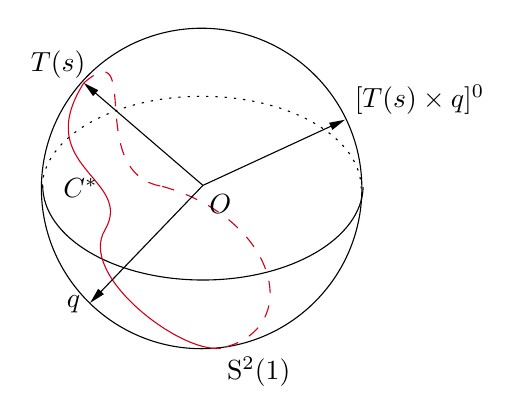
\begin{tikzpicture}[x=0.75pt,y=0.75pt,yscale=-1,xscale=1,scale=0.9]
			%uncomment if require: \path (0,300); %set diagram left start at 0, and has height of 300
			%Shape: Circle [id:dp9883588569540214] 
			\draw   (264.3,162.83) .. controls (264.3,115.45) and (302.71,77.05) .. (350.08,77.05) .. controls (397.46,77.05) and (435.86,115.45) .. (435.86,162.83) .. controls (435.86,210.2) and (397.46,248.61) .. (350.08,248.61) .. controls (302.71,248.61) and (264.3,210.2) .. (264.3,162.83) -- cycle ;
			%Shape: Arc [id:dp33661091255513176] 
			\draw  [draw opacity=0] (436.55,162.15) .. controls (435.68,189.68) and (397.61,211.84) .. (350.78,211.84) .. controls (303.41,211.84) and (265,189.16) .. (265,161.18) -- (350.78,161.18) -- cycle ; \draw   (436.55,162.15) .. controls (435.68,189.68) and (397.61,211.84) .. (350.78,211.84) .. controls (303.41,211.84) and (265,189.16) .. (265,161.18) ;
			%Shape: Arc [id:dp9245818042924343] 
			\draw  [draw opacity=0][dash pattern={on 0.84pt off 2.51pt}] (264.68,161.86) .. controls (265.58,135.05) and (303.47,113.48) .. (350.08,113.48) .. controls (397.26,113.48) and (435.5,135.57) .. (435.5,162.83) -- (350.08,162.83) -- cycle ; \draw  [dash pattern={on 0.84pt off 2.51pt}] (264.68,161.86) .. controls (265.58,135.05) and (303.47,113.48) .. (350.08,113.48) .. controls (397.26,113.48) and (435.5,135.57) .. (435.5,162.83) ;
			%Straight Lines [id:da35295309242701234] 
			\draw    (350.78,161.18) -- (288.51,107.66) ;
			\draw [shift={(287,106.35)}, rotate = 40.68] [fill={rgb, 255:red, 0; green, 0; blue, 0 }  ][line width=0.08]  [draw opacity=0] (8.4,-2.1) -- (0,0) -- (8.4,2.1) -- cycle    ;
			%Curve Lines [id:da7285876936925297] 
			\draw [color={rgb, 255:red, 208; green, 2; blue, 27 }  ,draw opacity=1 ] [dash pattern={on 4.5pt off 4.5pt}]  (287,106.35) .. controls (318.83,78.84) and (287,155.02) .. (329,161.69) ;
			%Curve Lines [id:da7078868094734088] 
			\draw [color={rgb, 255:red, 208; green, 2; blue, 27 }  ,draw opacity=1 ] [dash pattern={on 4.5pt off 4.5pt}]  (329,161.69) .. controls (391,179.02) and (405.66,238.35) .. (360.33,248.35) ;
			%Curve Lines [id:da2545979609312907] 
			\draw [color={rgb, 255:red, 208; green, 2; blue, 27 }  ,draw opacity=1 ]   (298.33,185.02) .. controls (314.43,157.58) and (258.33,151.69) .. (287,106.35) ;
			%Curve Lines [id:da9114196090867683] 
			\draw [color={rgb, 255:red, 208; green, 2; blue, 27 }  ,draw opacity=1 ]   (298.33,185.02) .. controls (283.66,209.02) and (338.43,251.18) .. (360.33,248.35) ;
			%Straight Lines [id:da691320506140914] 
			\draw    (350.78,161.18) -- (291.81,222.6) ;
			\draw [shift={(290.43,224.04)}, rotate = 313.84] [fill={rgb, 255:red, 0; green, 0; blue, 0 }  ][line width=0.08]  [draw opacity=0] (8.4,-2.1) -- (0,0) -- (8.4,2.1) -- cycle    ;
			%Straight Lines [id:da31732998081342445] 
			\draw    (350.78,161.18) -- (425.01,126.88) ;
			\draw [shift={(426.83,126.04)}, rotate = 155.2] [fill={rgb, 255:red, 0; green, 0; blue, 0 }  ][line width=0.08]  [draw opacity=0] (8.4,-2.1) -- (0,0) -- (8.4,2.1) -- cycle    ;

			% Text Node
			\draw (257.26,87.77) node [anchor=north west][inner sep=0.75pt]    {$\symbf{T}( s)$};
			% Text Node
			\draw (276.59,218.61) node [anchor=north west][inner sep=0.75pt]    {$\symbf{q}$};
			% Text Node
			\draw (430.67,105.78) node [anchor=north west][inner sep=0.75pt]    {$[\symbf{T}( s) \times \symbf{q}]^{0}$};
			% Text Node
			\draw (352.78,164.58) node [anchor=north west][inner sep=0.75pt]    {$O$};
			% Text Node
			\draw (274.67,156.11) node [anchor=north west][inner sep=0.75pt]    {$C^{*}$};
			% Text Node
			\draw (362.33,251.75) node [anchor=north west][inner sep=0.75pt]    {$\mathrm{S}^{2}( 1)$};


		\end{tikzpicture}
		\caption*{单位向量 $[\symbf{T}(s) \times \symbf{q}]^0$的构造}
		\label{切线像构造正交标架}
	\end{figure}
\end{frame}

\subsection{block}
\begin{frame}{定理环境}
	\begin{theorem}[Fenchel定理]
		$\mathbb{E}^3$ 中二阶连续可微闭曲线 $C$ 的全曲率
		$$
			K = \oint_C \kappa(s) \dif s \geqslant 2 \uppi,
		$$
		当且仅当 $C$ 为平面上的二阶连续可微凸闭曲线时等号成立.
	\end{theorem}
	\begin{proof}
		略.
	\end{proof}

\end{frame}
\begin{frame}{其他block样式}
	\begin{example}[高斯随机变量的尾分布]
		令$X\sim N(\mu,\sigma^2)$,则有
		\begin{equation}
			\mathbb{E}[\mathrm{e}^{\lambda x}]= \exp{\{\mu \lambda + \frac{\lambda^2\sigma^2}{2}\}}
		\end{equation}
		由Chernoff ineq., 有
		\begin{equation}
			\mathbb{P}(x-\mu \geqslant t) \leqslant \mathrm{e}^{-\frac{t^2}{2\sigma^2}}
			\label{高斯随机变量的尾分布}
		\end{equation}
	\end{example}
	\begin{alertblock}{注}
		其中\eqref{高斯随机变量的尾分布}式在一个多项式因子的修正后是sharp的.
	\end{alertblock}
\end{frame}

\section{致谢}
\begin{frame}
	\Huge
	$$
		\mathscr{THANKS}
	$$
\end{frame}
\end{document}
